
\section{Variational auto-encoder}


\begin{frame}{Variational auto-encoder}

Generative model with NN likelihood

~

\begin{columns}
	\begin{column}{0.2\textwidth}
	\begin{tikzpicture}
    % Define nodes
    \node[latent]		(z)		{$ z $};
    \node[obs, below = of z]		(x)		{$ x $};
    \node[right = of x]		(theta)		{$ \theta $};
    
    % Connect nodes
    \edge{z,theta}{x};
    
    % add plates
    \plate {x-sentence} {(x)(z)} {$ N $};
   
    \node[right = of z]		(lambda)		{$\phi $};   
    \edge[dashed, bend right]{x}{z};
    \edge[dashed]{lambda}{z};
    \end{tikzpicture}
    \end{column}
    \begin{column}{0.7\textwidth}
    	\begin{itemize}
			\item complex (non-linear) observation model $p_\theta(x|z)$
			\item complex (non-linear) mapping from data to latent variables $q_\phi(z|x)$
    	\end{itemize}
    \end{column}
    \end{columns}
    ~
    
    Jointly optimise generative model $p_\theta(x|z)$ and inference model $q_\phi(z|x)$ under the same objective (ELBO)
    
    \ack{\citet{KingmaWelling:2013}}
\end{frame}


\begin{frame}[plain]{Objective}

\begin{equation*}
\begin{aligned}
\log p_\theta(x) &\geq \overbrace{\E[q_\phi(z|x)]{\log p_\theta(x,z)} + \Ent{q_\phi(z|x)}}^{\ELBO} \\ 
\pause
&= \E[q_\phi(z|x)]{\log p_\theta(x|z) + \log p(z)} + \Ent{q_\phi(z|x)} \\ \pause
&= \E[q_\phi(z|x)]{\log p_\theta(x|z)} - \KL{q_\phi(z|x)}{p(z)}
\end{aligned}
\end{equation*}

\pause

Parameter estimation
\begin{equation*}
\argmax_{\theta,\phi} ~ \E[q_\phi(z|x)]{\log p_\theta(x|z)} - \KL{q_\phi(z|x)}{p(z)}
\end{equation*}

\pause

\begin{itemize}
	\item assume $\KL{q_\phi(z|x)}{p(z)}$  analytical\\
	true for exponential families \pause
	\item approximate $\E[q_\phi(z|x)]{\log p_\theta(x|z)}$ by sampling\\
	true because we design $q_\phi(z|x)$ to be simple
\end{itemize}


\end{frame}

\begin{frame}[plain]{Generative Network Gradient}
\begin{equation*}
\begin{aligned}
&\pdv{\theta} \left( \E[q_\phi(z|x)]{\log p_\theta(x|z)} - \overbrace{\KL{q_\phi(z|x)}{p(z)}}^{\text{constant wrt }\theta} \right) \\ \pause 
&=\underbrace{\E[q_\phi(z|x)]{\pdv{\theta}\log p_\theta(x|z)}}_{\text{expected gradient :)}} \\ \pause
&\overset{\text{MC}}{\approx} \frac{1}{K}\sum_{k=1}^{K}
\pdv{\theta} \log p_\theta(x|z^{(k)}) \\
&z^{(k)} \sim q_\phi(z|x)
\end{aligned}
\end{equation*}
\pause
\center{Note: $ q_\phi(z|x) $ does not depend on $ \theta $.}
\end{frame}

\begin{frame}{Inference Network Gradient}
\begin{equation*}
\begin{aligned}
&\pdv{\phi}\left(\E[q_\phi(z|x)]{\log p_\theta(x|z)} - \overbrace{\KL{q_\phi(z|x)}{p(z)}}^{\text{analytical}} \right) \\ \pause
=&\pdv{\phi}\E[q_\phi(z|x)]{\log p_\theta(x|z)} - \underbrace{\pdv{\phi}\KL{q_\phi(z|x)}{p(z)}}_{\text{analytical computation}} \\
\end{aligned}
\end{equation*}
\pause
The first term again requires approximation by sampling, \\
~ but there is a problem

\end{frame}

\begin{frame}{Inference Network Gradient}
\begin{equation*}
\begin{aligned}
&\pdv{\phi}\E[q_\phi(z|x)]{\log p_\theta(x|z)} \\ \pause
&= \pdv{\phi} \intl{q_\phi(z|x)\log p_\theta(x|z)}{z} \\ \pause
&=  \underbrace{\int \alert{\pdv{\phi}(q_\phi(z|x))}\log p_\theta(x|z) \dd{z}}_{\text{not an expectation}} 
\end{aligned}
\end{equation*}

\pause

\begin{itemize}
	\item MC estimator is non-differentiable: cannot sample first\\ \pause
	\item Differentiating the expression does not yield an expectation: cannot approximate via MC
\end{itemize}

\end{frame}

\begin{frame}{Score function estimator}

We can again use the log identity for derivatives
\begin{equation*}
\begin{aligned}
&\pdv{\phi}\E[q_\phi(z|x)]{\log p_\theta(x|z)} \\ 
&= \pdv{\phi} \intl{q_\phi(z|x)\log p_\theta(x|z)}{z} \\ 
&=  \underbrace{\int \alert{\pdv{\phi}(q_\phi(z|x))}\log p_\theta(x|z) \dd{z}}_{\text{not an expectation}} \\ \pause
&= \int \textcolor{blue}{q_\phi(z|x) \pdv{\phi}(\log q_\phi(z|x))} \log p_\theta(x|z) \dd{z} \\ \pause
&= \underbrace{\mathbb E_{q_\phi(z|x)} \left[  \log p_\theta(x|z)  \pdv{\phi}\log q_\phi(z|x)\right]}_{\text{expected gradient :)}}
\end{aligned}
\end{equation*}

\end{frame}

\begin{frame}[plain]{Score function estimator: high variance}


We can now build an MC estimator
\begin{equation*}
\begin{aligned}
&\pdv{\phi}\E[q_\phi(z|x)]{\log p_\theta(x|z)} \\ 
&= \mathbb E_{q_\phi(z|x)} \left[  \log p_\theta(x|z)  \pdv{\phi}\log q_\phi(z|x)\right] \\ \pause 
&\overset{\text{MC}}{\approx} \frac{1}{K} \sum_{k=1}^K \alert{\log p_\theta(x|z^{(k)})} \pdv{\phi}\log q_\phi(z^{(k)}|x) \\
&z^{(k)} \sim q_\phi(Z|x)
\end{aligned}
\end{equation*}

\pause
but
\begin{itemize}
	\item magnitude of $\log p_\theta(x|z)$ varies widely \pause 
	\item model likelihood does not contribute to direction of gradient \pause
	\item too much variance to be useful
\end{itemize}

\end{frame}

\begin{frame}{When variance is high we can}

\begin{itemize}
	\item sample more \\ \pause
	\alert{won't scale} \pause
	\item use variance reduction techniques (e.g. baselines and control variates)\\ \pause 		
	\item stare at this $\pdv{\phi}\E[q_\phi(z|x)]{\log p_\theta(x|z)}$ \\ \pause
	\textcolor{blue}{until we find a way to rewrite the expectation in terms of a density that 
	{\bf does not depend on} $\phi$}
\end{itemize}
\end{frame}

\begin{frame}{Reparametrisation}

Find a transformation $ h: z \mapsto \epsilon $ that expresses $z$ through a random variable $\epsilon$ such that \alert{ $q(\epsilon)$ does not depend on $\phi $} \pause
\begin{itemize}
\item $ h(z,\phi) $ needs to be invertible \pause
\item $ h(z,\phi) $ needs to be differentiable
\pause
\end{itemize}
Invertibility implies
\begin{itemize}
\item $ h(z,\phi) = \epsilon $
\item $ h^{-1}(\epsilon,\phi) = z $ 
\end{itemize}

\ack{\citep{KingmaWelling:2013,RezendeEtAl:2014,TitsiasLazarogredilla:2014}}

\end{frame}

\begin{frame}{Reparametrisation}
\begin{figure}
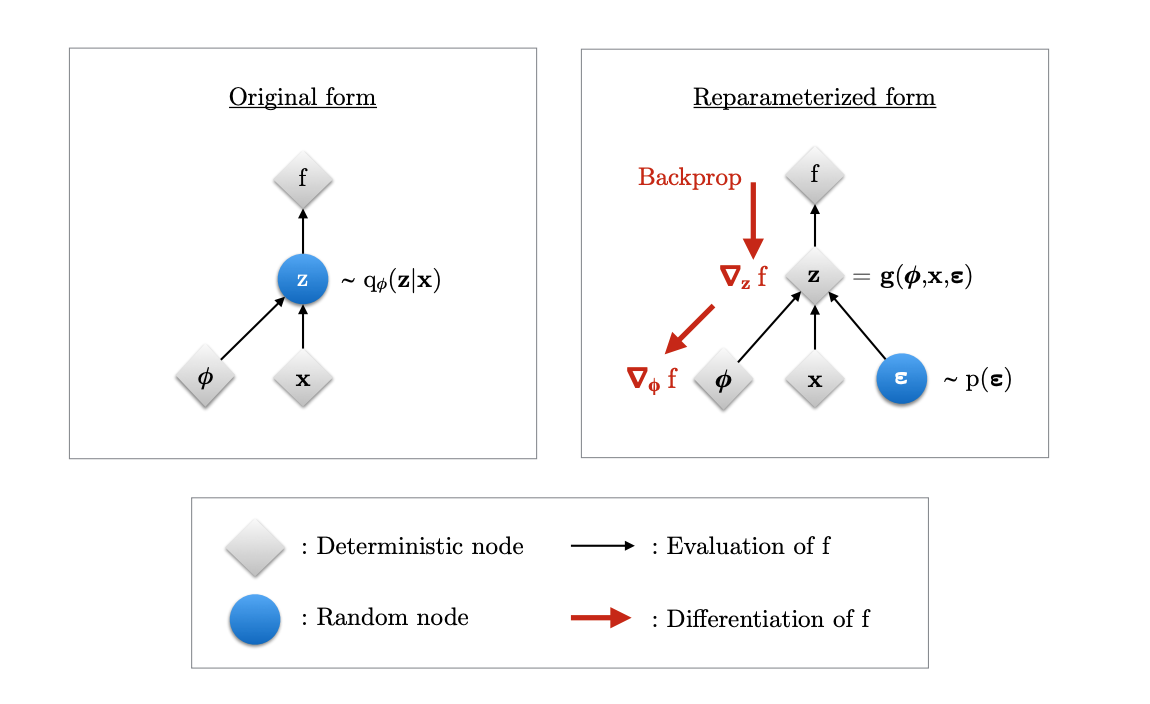
\includegraphics[scale=0.45]{rep_cg}
\end{figure}
\ack{\citep{KingmaWelling:2013}}
\end{frame}

\begin{frame}{Gaussian Transformation}

If $Z \sim \mathcal N(\mu_\phi(x), \sigma_\phi(x)^2)$ then

\begin{align*}
h(z,\phi) &= \frac{z - \mu_\phi(x)}{ \sigma_\phi(x) } = \epsilon \sim \NDist{0}{\IMatrix} \\
h^{-1}(\epsilon,\phi) &= \mu_\phi(x) + \sigma_\phi(x) \odot \epsilon~~~\epsilon \sim \NDist{0}{\IMatrix}
\end{align*}


\end{frame}

\begin{frame}[plain]{Inference Network -- Reparametrised Gradient}

\begin{equation*}
\begin{aligned}
&= \pdv{\phi} \int q_\phi(z|x)\log p_\theta(x|z) \dd{z} \\ \pause
&= \pdv{\phi} \int \alert{q(\epsilon)} \log p_\theta(x | \alert{\overbrace{h^{-1}(\epsilon,\phi)}^{=z}}) \dd{\alert{\epsilon}} \\ \pause
&= \int q(\epsilon) \pdv{\phi} \left[ \log p_\theta(x| \overbrace{h^{-1}(\epsilon,\phi)}^{=z})\right] \dd{\epsilon} \\ \pause
&= \underbrace{\mathbb E_{q(\epsilon)}\left[ \pdv{\phi} \log p_\theta(x| h^{-1}(\epsilon,\phi))\right] \dd{\epsilon}}_{\text{expected gradient :D}} 
%&= \int q(\epsilon) \underbrace{\pdv{z} \log p_\theta(x| h^{-1}(\epsilon,\phi)) \times \pdv{\phi} h^{-1}(\epsilon,\phi)}_{\text{chain rule}} \dd{\epsilon}  \\ \pause
%&= \mathbb E_{q(\epsilon)} \left[ \underbrace{\pdv{z} \log p_\theta(x| \overbrace{h^{-1}(\epsilon,\phi)}^{=z}) \times \pdv{\phi} h^{-1}(\epsilon,\phi)}_{\text{chain rule}} \right]
\end{aligned}
\end{equation*}
\end{frame}

\begin{frame}[plain]{Reparametrised gradient estimate}

\begin{equation*}
\begin{aligned}
&= \underbrace{\mathbb E_{q(\epsilon)}\left[ \pdv{\phi} \log p_\theta(x| h^{-1}(\epsilon,\phi))\right] \dd{\epsilon}}_{\text{expected gradient :D}} \\ \pause
&= \mathbb E_{q(\epsilon)} \left[ \underbrace{\pdv{z} \log p_\theta(x| \overbrace{h^{-1}(\epsilon,\phi)}^{=z}) \times \pdv{\phi} h^{-1}(\epsilon,\phi)}_{\text{chain rule}} \right] \\ \pause
&\overset{\text{MC}}{\approx} \frac{1}{K}\sum_{k=1}^{K} \underbrace{\pdv{z} \log p_\theta(x| \overbrace{h^{-1}(\epsilon^{(k)},\phi)}^{=z}) \times \pdv{\phi} h^{-1}(\epsilon^{(k)},\phi)}_{\text{backprop's job}}\\
&\epsilon^{(k)} \sim q(\epsilon)
\end{aligned}
\end{equation*}

Note that both models contribute with gradients

\end{frame}

\begin{frame}{Gaussian KL}
\begin{block}{ELBO}
\begin{equation*}
\E[q_\phi(z|x)]{\log p_\theta(x|z)} - \KL{q_\phi(z|x)}{p(z)}
\end{equation*}
\end{block}
\pause
Analytical computation of $ -\KL{q_\phi(z|x)}{p(z)} $:
\begin{equation*}
\frac{1}{2}\sum_{i=1}^{d}\left(1 + \loga{\sigma^{2}_{i}} -
\mu^{2}_{i} - \sigma^{2}_{i} \right)
\end{equation*}
\pause
Thus backprop will compute $-\pdv{\phi} \KL{q_\phi(z|x)}{p(z)}$ for us
\end{frame}

\begin{frame}{Computation Graph}
\begin{figure}
\begin{tikzpicture}[node distance=1cm]
\node[rectangle, draw, rounded corners, thick] (input) {$x$};
\node[rectangle, draw, rounded corners, thick, above left=of input] (mu) {$ \mu $};
\node[rectangle, draw, rounded corners, thick, above right=of input] (var) {$ \sigma $};
\node[rectangle, draw, rounded corners, thick, above right= of mu] (z) {$ z $};
\node[rectangle, fill=blue!20, thick, above of= z, rounded corners, draw, node distance=1.5cm] (output) {$ x $};

\draw[->, thick] (input) -- (mu) node[midway, above, rotate=315] {$\phi $};
\draw[->, thick] (input) -- (var) node[midway, above, rotate=45] {$\phi $};
\draw[->, thick] (mu) edge (z);
\draw[->, thick] (var) edge (z);
\draw[->, thick] (z) -- (output) node[midway, right] {$ \theta $};

\pause
\node[draw=orange, thick, rectangle, fit= (input) (mu) (var), rounded corners] {};
\node[left= of mu] (inference) {\textcolor{orange}{inference model}};

\pause
\node[draw=blue!50, thick, rectangle, fit= (z) (output), rounded corners] {};
\node[above= of inference] (generation) {\textcolor{blue!50}{generative model}};

\pause
\node[circle, draw, thick ,right =of var, xshift=-.5cm] (epsilon) {$ \epsilon $};
\node[right = of epsilon, xshift=-1cm] (stdNormal) {$ \sim \NDist{0}{1} $};
\draw[->, thick] (epsilon) edge (var);

\pause
\node[above= of mu, rectangle, fill=blue!20, thick, rounded corners, draw,] (KLmu) {$ \KullbackLeibler $};
\draw[->, thick] (mu) edge (KLmu);
\node[above= of var, rectangle, fill=blue!20, thick, rounded corners, draw,] (KLvar) {$ \KullbackLeibler $};
\draw[->, thick] (var) edge (KLvar);
\end{tikzpicture}
\end{figure}
\end{frame}

\begin{frame}{Example}
	\begin{tikzpicture}
    % Define nodes
    \node[latent]		(z)		{$ z $};
    \node[obs, right = of z]		(x)		{$ x_1^m $};
    \node[right = of x]		(theta)		{$ \theta $};
    
    % Connect nodes
    \edge{z,theta}{x};
    
    % add plates
    \plate {x-sentence} {(x)(z)} {$ N $};
   
    \node[left = of z]		(lambda)		{$\phi $};   
    \edge[dashed, bend right]{x}{z};
    \edge[dashed]{lambda}{z};
    \end{tikzpicture}

	Generative model
    	\begin{itemize}
			\item $Z \sim \mathcal N(0, I)$
			\item $X_i | z, x_{<i} \sim \Cat(f_\theta(z, x_{<i}))$\\
			%where $x_{<i}$ is represented by a recurrent hidden state\\
			%and the categorical parameters are predicted by a single hidden layer FFNN with softmax activation
    	\end{itemize}
	Inference model
    	\begin{itemize}
			\item $Z \sim \mathcal N(\mu_\phi(x_1^m), \sigma_\phi(x_1^m)^2)$
			%where $x_1^m$ is represented by the average embedding\\
			%location and scale are single hidden layer FFNNs
    	\end{itemize}
	
	
	\ack{\citet{bowman-EtAl:2016}}
	
\end{frame}



\begin{frame}{VAEs -- Summary}
\textbf{Advantages}
\begin{itemize}
\item Backprop training
\item Easy to implement
\item Posterior inference possible
\item One objective for both NNs
\end{itemize}
\pause
\textbf{Drawbacks}
\begin{itemize}
\item Discrete latent variables are difficult
\item Optimisation may be difficult with several latent variables
\item Location-scale families only\\
but see \citet{RuizEtAl:2016} and \citet{KucukelbirEtAl:2017}
\end{itemize}
\end{frame}

\subsection{Semi supervised VAE}

\begin{frame}{Semi-supervised VAE}
\begin{figure}
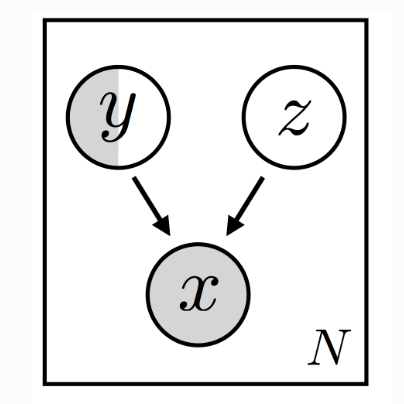
\includegraphics[scale=0.45]{semi-sup}
\end{figure}
\ack{\citep{NIPS2014_5352}}
\end{frame}

\begin{frame}{Semi-supervised VAE}

\begin{itemize}
\item Generative model:
\begin{equation}
\begin{aligned}
p(y)=\operatorname{cat}(y | \boldsymbol{\pi}) ;\\
\quad p(\mathbf{z})=\mathcal{N}(\mathbf{z} | \mathbf{0}, \mathbf{I}) ;\\
\quad p_{\theta}(\mathbf{x} | y, \mathbf{z})=f(\mathbf{x} ; y, \mathbf{z}, \boldsymbol{\theta})
\end{aligned}
\end{equation}
\item Inference model:
\begin{equation}
\begin{aligned}
q_{\phi}(\mathbf{z} | y, \mathbf{x})=\mathcal{N}\left(\mathbf{z} | \boldsymbol{\mu}_{\phi}(y, \mathbf{x}), \operatorname{diag}\left(\boldsymbol{\sigma}_{\phi}^{2}(\mathbf{x})\right)\right) ; \\
q_{\phi}(y | \mathbf{x})=\operatorname{Cat}\left(y | \boldsymbol{\pi}_{\phi}(\mathbf{x})\right)
\end{aligned}
\end{equation}
\end{itemize}
\end{frame}

\begin{frame}{Objective}
\footnotesize{
\begin{itemize}

\item Labelled data: \\
\begin{equation}
\begin{aligned}
\log p_{\theta}(\mathbf{x}, y) \geq & \mathbb{E}_{q_{\phi}(\mathbf{z} | \mathbf{x}, y)}\left[\log p_{\theta}(\mathbf{x} | y, \mathbf{z})+\log p_{\theta}(y)+\log p(\mathbf{z})-\log q_{\phi}(\mathbf{z} | \mathbf{x}, y)\right]
= & -\mathcal{L}(\mathbf{x}, y)
\end{aligned}
\end{equation}
\item Unlabelled data: \\
\begin{equation}
\begin{aligned} 
\log p_{\theta}(\mathbf{x}) & \geq \mathbb{E}_{q_{\phi}(y, \mathbf{z} | \mathbf{x})}\left[\log p_{\theta}(\mathbf{x} | y, \mathbf{z})+\log p_{\theta}(y)+\log p(\mathbf{z})-\log q_{\phi}(y, \mathbf{z} | \mathbf{x})\right] \\ 
&=\sum_{y} q_{\phi}(y | \mathbf{x})(-\mathcal{L}(\mathbf{x}, y))+\mathcal{H}\left(q_{\phi}(y | \mathbf{x})\right)=-\mathcal{U}(\mathbf{x})
\end{aligned}
\end{equation}
\end{itemize}
}
\end{frame}


\subsection{Beyond mean field}

\begin{frame}{Beyond the mean field}
\begin{figure}
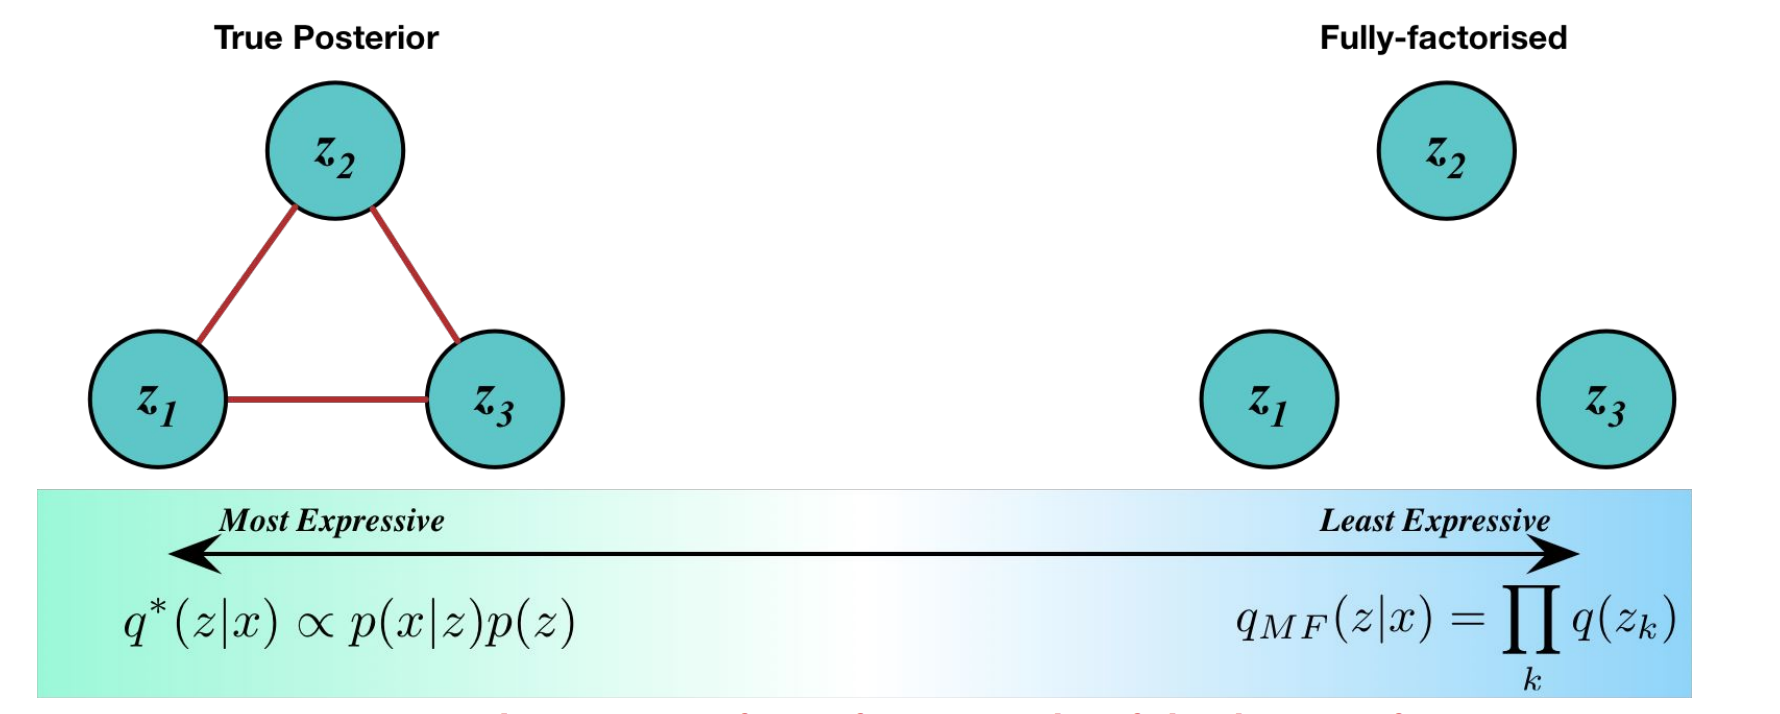
\includegraphics[scale=0.25]{struct2meanfield}
\end{figure}
\ack{Mohamed S. 2017, Deep Generative Models Tutorial}
\end{frame}

\begin{frame}{Auxiliary variable}
The mean field assumption might result in models that do not capture all dependencies in the observations:\\

\begin{figure}
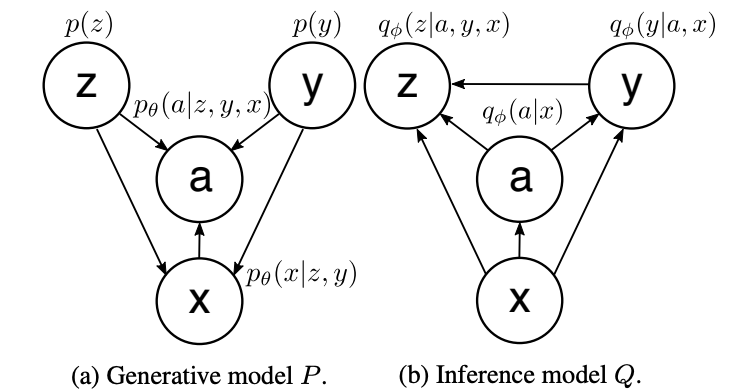
\includegraphics[scale=0.45]{aux_variable2}
\end{figure}
\ack{\citep{pmlr-v48-maaloe16}}
\end{frame}

\begin{frame}{Auxiliary variable}
\begin{itemize}
\item Generative model: \\
\begin{equation}
\begin{aligned}
p(z) &=\mathcal{N}(z | 0, \mathrm{I}) \\ p(y) &=\operatorname{Cat}(y | \pi) \\ p_{\theta}(a | z, y, x) &=f(a ; z, y, x, \theta) \\ p_{\theta}(x | z, y) &=f(x ; z, y, \theta) 
\end{aligned}
\end{equation}
\item Inference model: \\
\begin{equation}
\begin{aligned}
 q_{\phi}(a | x) &=\mathcal{N}\left(a | \mu_{\phi}(x), \operatorname{diag}\left(\sigma_{\phi}^{2}(x)\right)\right) \\
  q_{\phi}(y | a, x) &=\operatorname{Cat}\left(y | \pi_{\phi}(a, x)\right) \\ 
  q_{\phi}(z | a, y, x) &=\mathcal{N}\left(z | \mu_{\phi}(a, y, x), \operatorname{diag}\left(\sigma_{\phi}^{2}(a, y, x)\right)\right) 
 \end{aligned}
\end{equation}
\end{itemize}
\end{frame}


\begin{frame}{Normalizing flow}
\begin{figure}
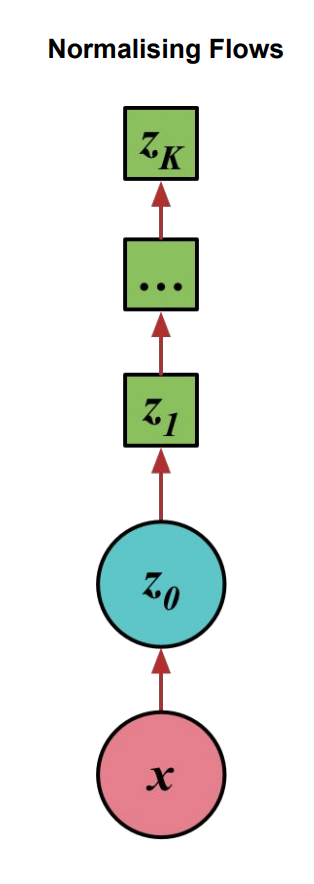
\includegraphics[scale=0.35]{NF}
\end{figure}
\end{frame}

\begin{frame}{NF for NLP}
\begin{itemize}
\item \citep{effective2019pelsmaeker} tackle issues present in VAE models for language.
\item Annealing
\item Expressive posterior
\end{itemize}
\end{frame}

